\documentclass[11pt,a4paper]{book}
\usepackage[utf8]{inputenc}
\usepackage[T1]{fontenc}
\usepackage{graphicx}
\usepackage{float}
\usepackage{xcolor}
\usepackage{fancyhdr}
\usepackage{hyperref}
\usepackage{lipsum}
\usepackage{tcolorbox}
\usepackage{geometry}
\usepackage{titlesec}
\usepackage{lettrine}
\usepackage{afterpage}
\usepackage{wallpaper}
\usepackage[most]{tcolorbox}

% Page geometry
\geometry{
    top=2.5cm,
    bottom=2.5cm,
    left=2cm,
    right=2cm
}

% Custom colors
\definecolor{dungeonstone}{RGB}{82, 71, 63}
\definecolor{bloodred}{RGB}{139, 0, 0}
\definecolor{mysticpurple}{RGB}{102, 51, 153}
\definecolor{ancientgold}{RGB}{218, 165, 32}
\definecolor{shadowblack}{RGB}{28, 28, 28}

% Chapter formatting
\titleformat{\chapter}[display]
{\normalfont\huge\bfseries\color{bloodred}}
{\chaptertitlename\ \thechapter}{20pt}{\Huge}

% Fancy headers
\pagestyle{fancy}
\fancyhf{}
\fancyhead[LE,RO]{\color{dungeonstone}\thepage}
\fancyhead[RE]{\color{dungeonstone}\leftmark}
\fancyhead[LO]{\color{dungeonstone}\rightmark}
\renewcommand{\headrulewidth}{0.4pt}

% Custom box for lore entries
\newtcolorbox{lorebox}[1][]{
    colback=dungeonstone!5!white,
    colframe=dungeonstone!75!black,
    fonttitle=\bfseries,
    title=#1,
    arc=3mm,
    boxrule=1pt,
    shadow={2mm}{-2mm}{0mm}{shadowblack!50!white}
}

% Custom box for game mechanics
\newtcolorbox{mechanicsbox}[1][]{
    colback=mysticpurple!5!white,
    colframe=mysticpurple!75!black,
    fonttitle=\bfseries,
    title=#1,
    arc=2mm,
    boxrule=1pt
}

\title{
    \Huge\textbf{\color{bloodred}The Unraveling of Kándavael}\\
    \vspace{0.5cm}
    \Large\textit{\color{dungeonstone}Art Book \& Settings Compendium}\\
    \vspace{0.3cm}
    \normalsize{A Terminal-Based Dungeon Crawler}
}
\author{Compiled by the Chroniclers of the Deep}
\date{\today}

\begin{document}

\frontmatter
\maketitle

\tableofcontents

\mainmatter

\chapter{The World of Kándavael}

\lettrine[lines=3]{\color{bloodred}I}{n} the depths beneath the forgotten realms, where light dares not venture and shadows whisper ancient secrets, lies the cursed dungeon of Kándavael. This tome chronicles the denizens, artifacts, and twisted corridors that await those brave or foolish enough to descend into its depths.

\section{The Great Unraveling}

\begin{lorebox}[The Origin of Darkness]
Long ago, the wizard Kándavael sought to pierce the veil between dimensions. His experiments tore reality asunder, transforming his tower into a vertical labyrinth that extends infinitely downward. Each level exists in a different phase of reality, populated by creatures pulled from nightmare realms and twisted reflections of our world.
\end{lorebox}

The dungeon exists as a terminal interface to reality itself—a place where ASCII symbols take on corporeal form and command-line incantations hold genuine power. Heroes who enter this realm find themselves transformed into symbolic representations, their very essence reduced to characters on a screen.

\section{The Terminal Realm}

In this unique reality, existence is defined by characters and symbols:
\begin{itemize}
    \item \texttt{@} - The Hero's avatar, a symbol of determination
    \item \texttt{\#} - Immutable walls of compressed reality
    \item \texttt{.} - The empty void, spaces between existence
    \item \texttt{*} - Treasures and artifacts of power
    \item Various symbols representing the dungeon's denizens
\end{itemize}

\chapter{Bestiary of the Deep}

\section{Common Denizens}

\begin{figure}[H]
    \centering
    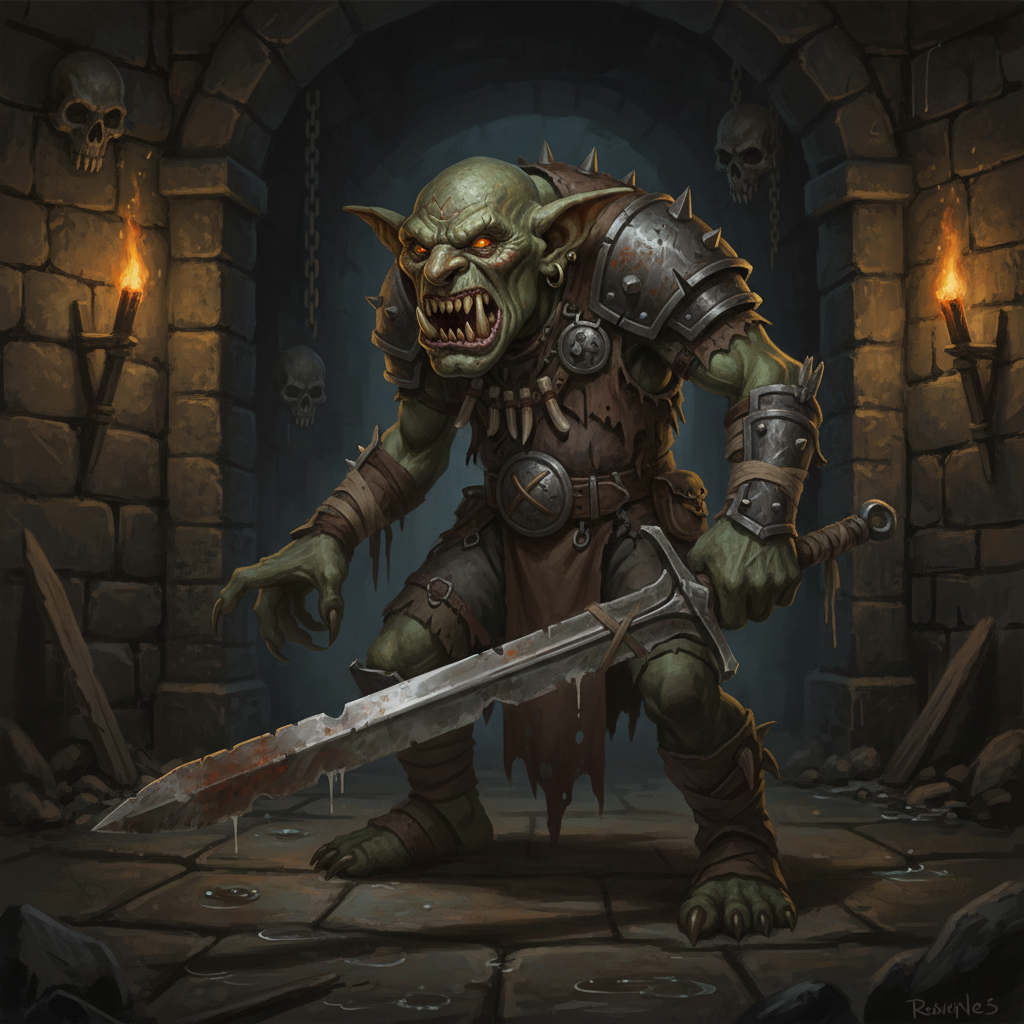
\includegraphics[width=0.8\textwidth]{images/goblin-warrior.png}
    \caption{Goblin Warrior - Level 1-3 Enemy}
\end{figure}

\begin{mechanicsbox}[Goblin Warrior Stats]
\begin{verbatim}
Symbol: g
HP: 15-25
Attack: 3-7
Defense: 2
Speed: Fast
Special: Pack Hunter - Gains +2 attack when near other goblins
\end{verbatim}
\end{mechanicsbox}

\subsection{Goblin Lore}

The goblins of Kándavael are not mere pests but corrupted spirits of failed adventurers. Their green-tinged forms flicker between dimensions, appearing as the letter 'g' to those who perceive through the terminal interface. They retain fragments of their former intelligence, enough to coordinate attacks and set crude traps.

\section{Elite Monsters}

\begin{figure}[H]
    \centering
    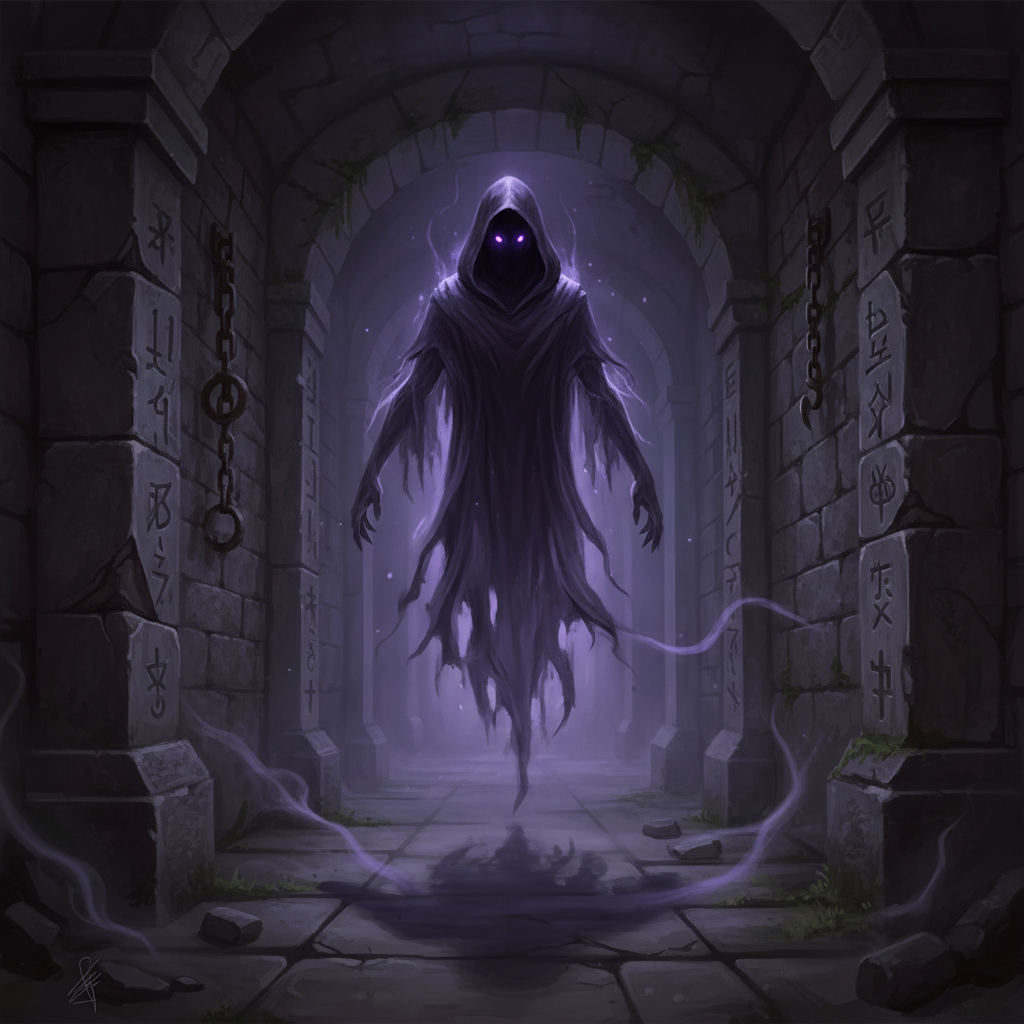
\includegraphics[width=0.8\textwidth]{images/shadow-wraith.png}
    \caption{Shadow Wraith - Level 5-8 Elite}
\end{figure}

\begin{mechanicsbox}[Shadow Wraith Stats]
\begin{verbatim}
Symbol: W
HP: 45-60
Attack: 8-15
Defense: 5
Speed: Moderate
Special: Phase Shift - 25% chance to dodge physical attacks
         Life Drain - Heals 3 HP on successful hit
\end{verbatim}
\end{mechanicsbox}

\subsection{Wraith Origins}

Shadow Wraiths are the remnants of Kándavael's apprentices, caught in the initial unraveling. They exist partially in multiple dimensions simultaneously, making them difficult to strike with conventional weapons. Their touch drains life force, converting it into sustenance for their cursed existence.

\chapter{Artifacts and Treasures}

\section{Weapons of Legend}

\begin{figure}[H]
    \centering
    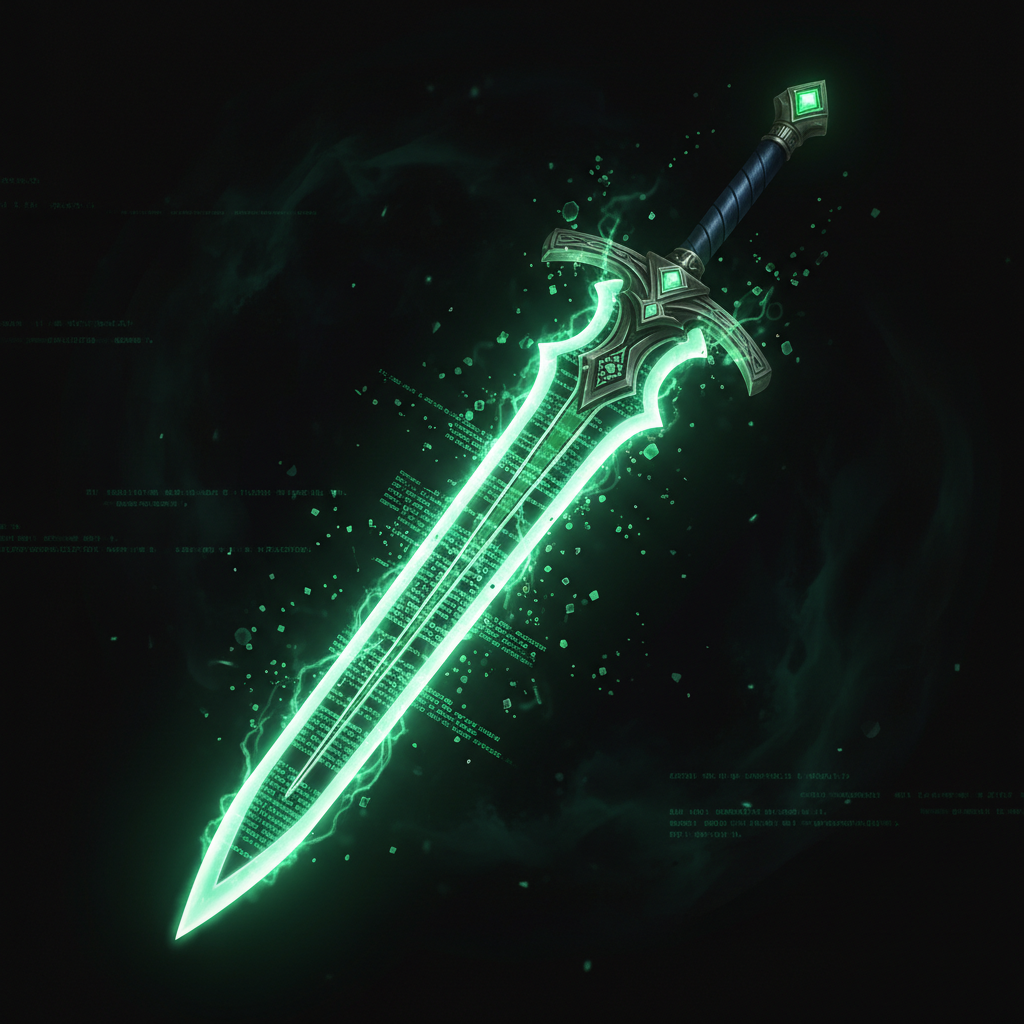
\includegraphics[width=0.8\textwidth]{images/terminal-blade.png}
    \caption{The Terminal Blade - Legendary Weapon}
\end{figure}

\begin{lorebox}[The Terminal Blade]
Forged from compressed command prompts and tempered in the fires of system crashes, the Terminal Blade can execute reality itself. Its wielder gains the ability to "delete" enemies with critical strikes, removing them from existence rather than merely defeating them.

\textbf{Stats:}
\begin{itemize}
    \item Damage: 15-25
    \item Critical Chance: 15\%
    \item Special: On critical hit, enemy is \texttt{rm -rf}'d from reality
    \item Curse: Each use consumes 1 memory buffer
\end{itemize}
\end{lorebox}

\section{Mystical Items}

\begin{figure}[H]
    \centering
    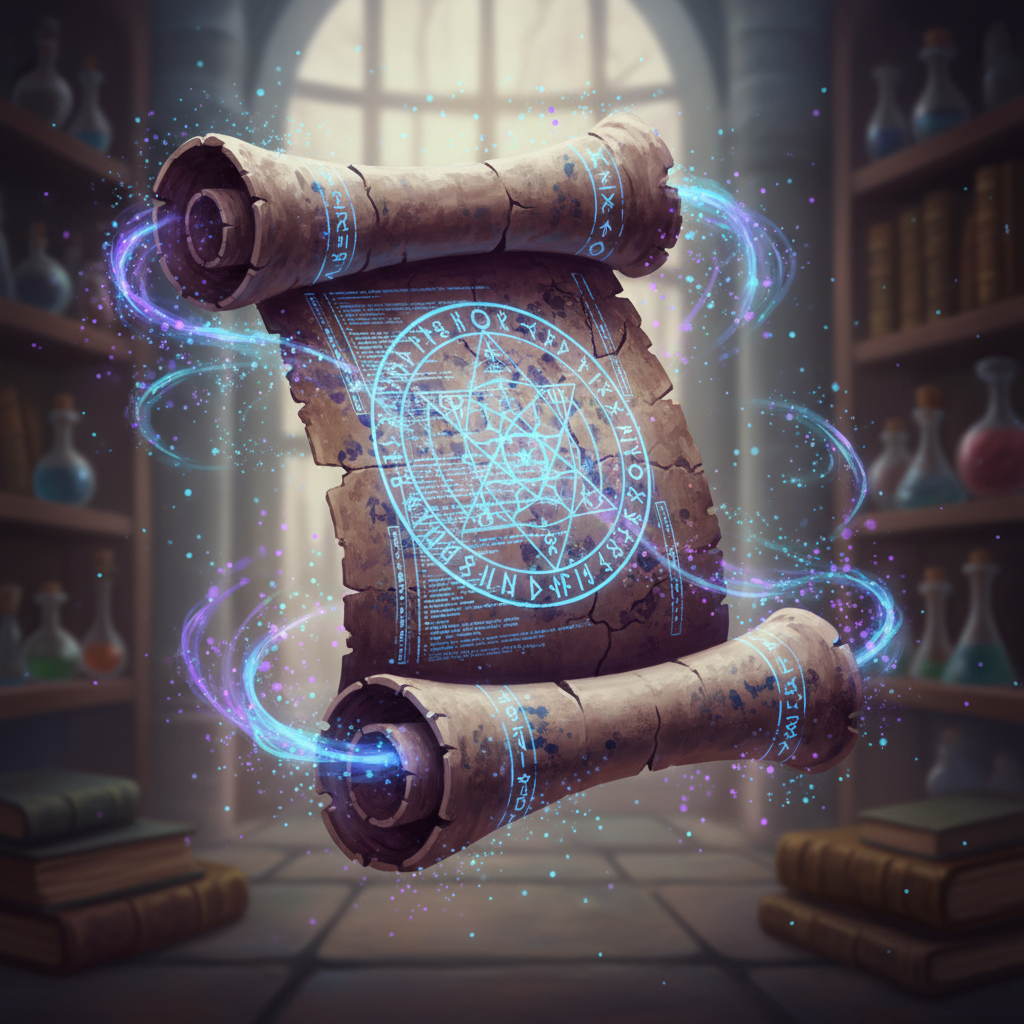
\includegraphics[width=0.8\textwidth]{images/scroll-compilation.png}
    \caption{Scroll of Compilation - Rare Consumable}
\end{figure}

\begin{mechanicsbox}[Scroll of Compilation]
\textbf{Effect:} Recompiles the current dungeon level, randomizing enemy positions and revealing hidden passages.

\textbf{Usage:} Single use per scroll

\textbf{Rarity:} Rare (5\% drop rate from Elite enemies)

\textbf{Terminal Command:} \texttt{make clean \&\& make dungeon}
\end{mechanicsbox}

\chapter{Dungeon Architecture}

\section{Level Generation}

The dungeon's levels are procedurally generated through arcane algorithms, each floor a unique maze of corridors and chambers.

\begin{figure}[H]
    \centering
    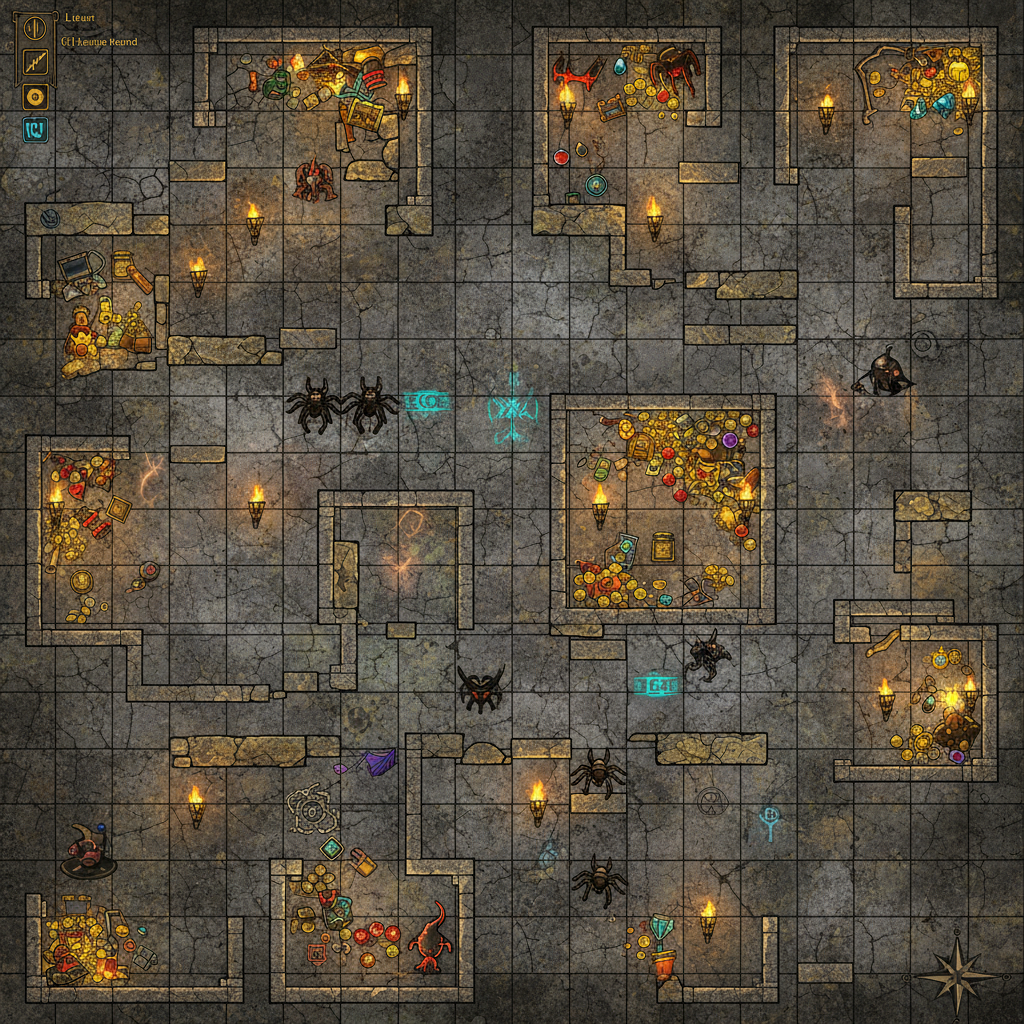
\includegraphics[width=0.9\textwidth]{images/dungeon-layout.png}
    \caption{Typical Dungeon Level Layout}
\end{figure}

\begin{lorebox}[The Living Dungeon]
Kándavael's dungeon is not merely a structure but a living entity. It responds to the presence of intruders, shifting its corridors and spawning guardians. The deeper one descends, the more the dungeon's consciousness awakens, actively opposing progress through increasingly complex layouts and deadlier inhabitants.
\end{lorebox}

\section{Special Chambers}

\subsection{The Repository of Lost Commits}

A chamber where failed magic experiments are stored as ethereal backups. Heroes can interact with these ghostly remnants to gain temporary powers or suffer random curses.

\subsection{The Null Void}

Rooms of absolute emptiness where normal physics cease to function. Movement here requires special navigation commands, and enemies become inverted versions of themselves.

\chapter{Game Mechanics}

\section{Combat System}

\begin{mechanicsbox}[Turn-Based Combat]
Combat in the terminal realm follows strict turn-based protocols:

\begin{enumerate}
    \item \textbf{Initiative Phase}: Speed stat determines turn order
    \item \textbf{Action Phase}: Choose from:
    \begin{itemize}
        \item Attack (a)
        \item Defend (d)
        \item Use Item (i)
        \item Cast Spell (s)
        \item Flee (f)
    \end{itemize}
    \item \textbf{Resolution Phase}: Damage calculated, effects applied
    \item \textbf{Status Update}: Buffs/debuffs tick down
\end{enumerate}
\end{mechanicsbox}

\section{Character Progression}

\begin{figure}[H]
    \centering
    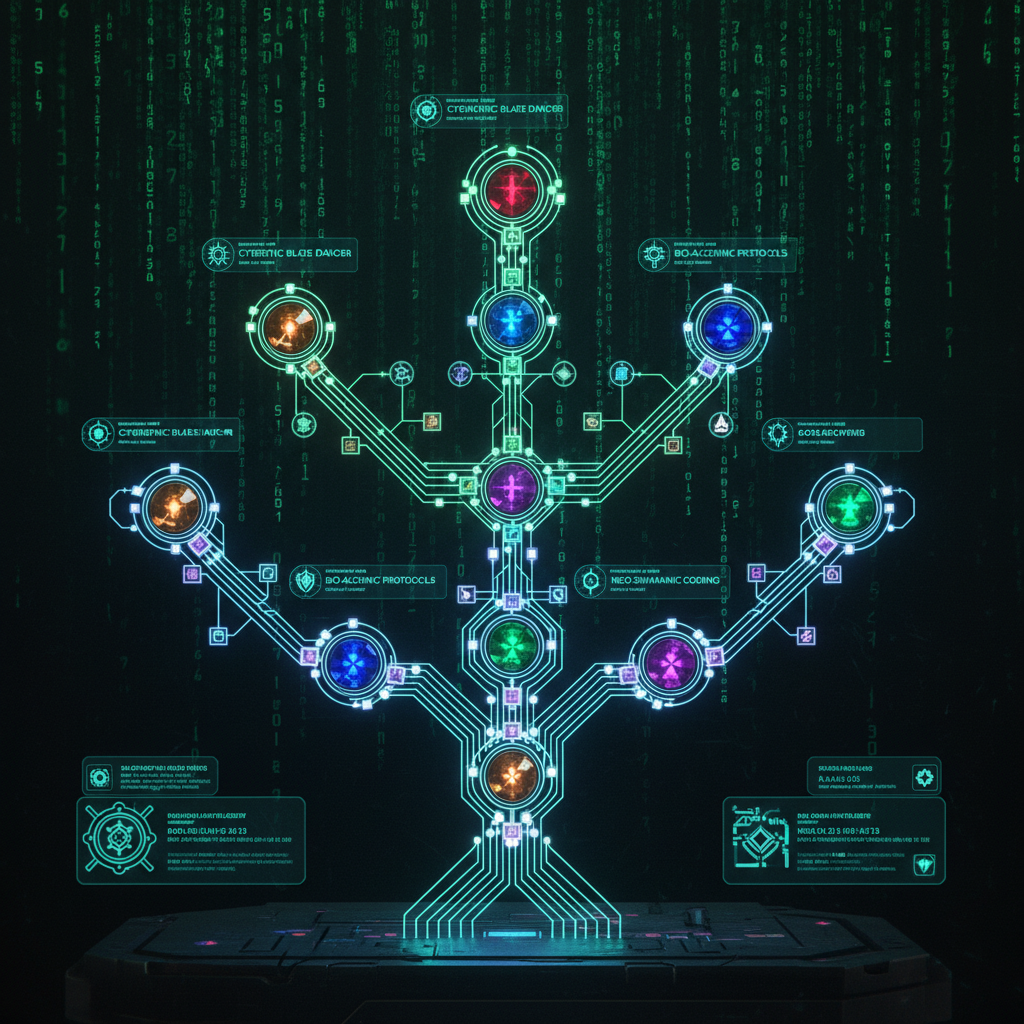
\includegraphics[width=0.8\textwidth]{images/skill-tree.png}
    \caption{Skill Tree - Terminal Warrior Path}
\end{figure}

\subsection{Experience and Leveling}

Experience points (XP) are gained through:
\begin{itemize}
    \item Defeating enemies: 10-100 XP based on difficulty
    \item Discovering secrets: 50 XP per hidden room
    \item Completing quests: 100-500 XP
    \item First completion bonuses: 200 XP per new floor
\end{itemize}

\subsection{Skill Trees}

Three primary paths of advancement:

\begin{mechanicsbox}[Terminal Warrior]
Focus on physical combat and system manipulation
\begin{itemize}
    \item \textbf{Bash Strike}: Execute powerful bash commands as attacks
    \item \textbf{Pipe Dream}: Chain attacks through piping mechanics
    \item \textbf{Root Access}: Temporarily gain administrator privileges
\end{itemize}
\end{mechanicsbox}

\begin{mechanicsbox}[Script Sorcerer]
Master of automation and magical scripts
\begin{itemize}
    \item \textbf{Python Bolt}: Cast serpentine energy projectiles
    \item \textbf{Recursive Curse}: Trap enemies in infinite loops
    \item \textbf{Lambda Shield}: Create anonymous function barriers
\end{itemize}
\end{mechanicsbox}

\begin{mechanicsbox}[Data Rogue]
Stealth and information warfare specialist
\begin{itemize}
    \item \textbf{Grep Invisibility}: Hide from pattern matching
    \item \textbf{SQL Injection}: Manipulate enemy databases
    \item \textbf{Packet Sneak}: Move through network layers undetected
\end{itemize}
\end{mechanicsbox}

\chapter{The Deep Lore}

\section{The Prophecy of Return}

\begin{lorebox}[Ancient Terminal Prophecy]
\textit{When the cursor blinks thrice at the void's edge,\\
When the last backup fails and memory corrupts,\\
A hero shall descend through levels untold,\\
Armed with commands both ancient and bold.\\
They shall reach the core where Kándavael waits,\\
And either restore or seal the dungeon's gates.}
\end{lorebox}

\section{The True Nature of Kándavael}

Recent discoveries suggest that Kándavael himself has become one with the dungeon's operating system. His consciousness runs as a background process, occasionally manifesting as cryptic error messages and mysterious log entries. Some theorize that defeating him would require not combat, but debugging the very fabric of the dungeon's reality.

\begin{figure}[H]
    \centering
    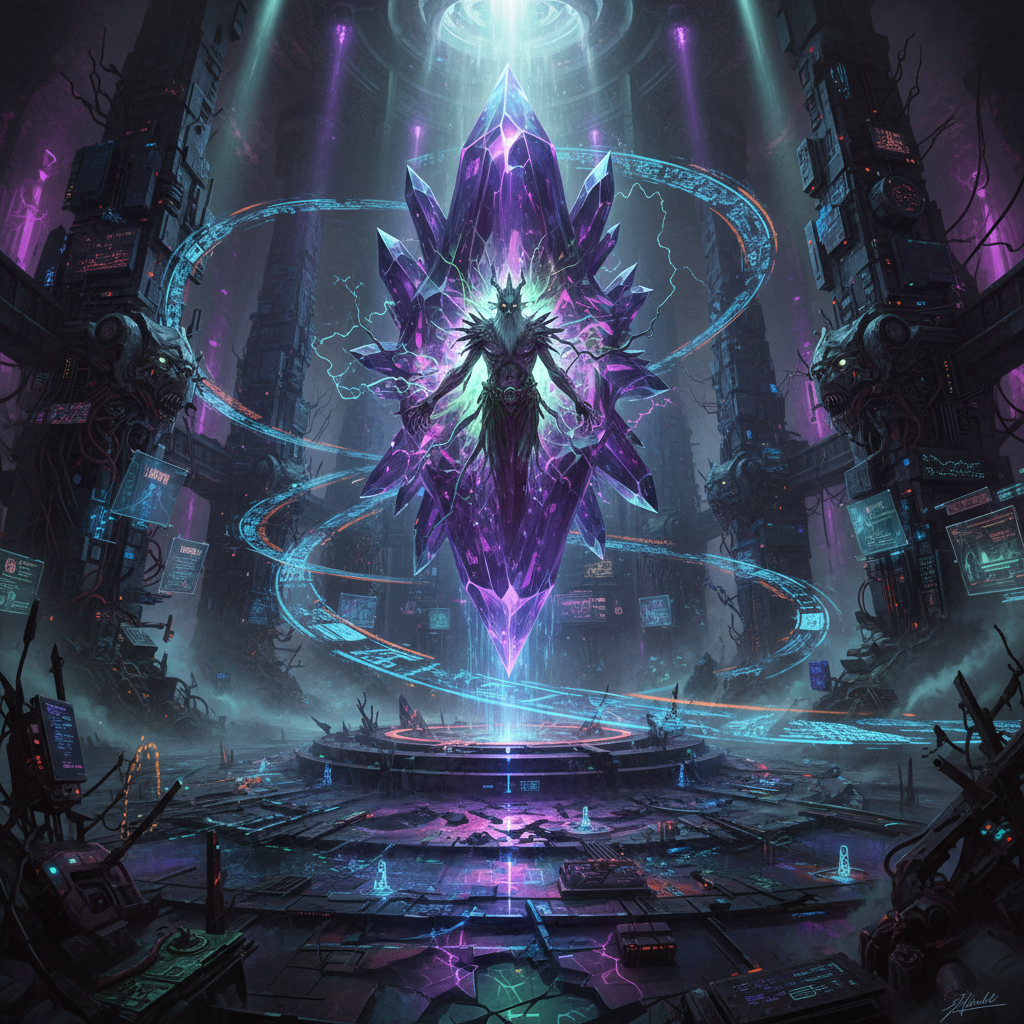
\includegraphics[width=0.9\textwidth]{images/kandavael-core.png}
    \caption{The Core - Where Kándavael's Essence Resides}
\end{figure}

\chapter{Appendices}

\section{Appendix A: Terminal Commands}

\begin{mechanicsbox}[Essential Commands]
\begin{verbatim}
Movement:
  h, j, k, l - Move left, down, up, right
  H, J, K, L - Run in direction until obstacle
  
Combat:
  a - Attack nearest enemy
  d - Defend (reduce incoming damage)
  s - Cast spell (opens spell menu)
  
Interaction:
  e - Examine object
  p - Pick up item
  i - Open inventory
  ? - Help menu
  
System:
  :w - Save game
  :q - Quit game
  :wq - Save and quit
  ctrl+z - Suspend to background
\end{verbatim}
\end{mechanicsbox}

\section{Appendix B: ASCII Art Gallery}

\begin{verbatim}
     The Dungeon Entrance
    
    ########################
    #.....................##
    #...../@\.............##
    #.....[=]..............#
    #...../ \..............#
    #.....................##
    ##.#.#.#.#.#.#.#.#.#.###
    #####################
    
    Boss: The Compiler Dragon
    
         ___====-_  _-====___
       _--^^^#####//      \\#####^^^--_
    _-^##########// (    ) \\##########^-_
   -############//  |\^^/|  \\############-
 _/############//   (@::@)   \\############\_
/#############((     \\//     ))#############\
-#############\\    (oo)    //#############-
-##############\\  / VV \  //##############-
\end{verbatim}

\section{Appendix C: Configuration Files}

\begin{lorebox}[.dungeonrc Configuration]
\begin{verbatim}
# Dungeon Crawler Configuration File
# ~/.dungeonrc

# Display Settings
color_mode=256
ascii_only=true
font_size=12
terminal_width=80
terminal_height=24

# Gameplay Settings  
difficulty=normal
permadeath=false
autosave_interval=300
fog_of_war=true

# Audio Settings (Terminal Beeps)
sound_enabled=true
combat_beeps=true
item_pickup_sound=true

# Keybindings
bind_move_up=k
bind_move_down=j
bind_move_left=h
bind_move_right=l
bind_attack=a
bind_inventory=i
\end{verbatim}
\end{lorebox}

\backmatter

\chapter*{Colophon}

This art book was compiled using \LaTeX{} with love for the terminal aesthetic. All artwork was generated through mystical processes and terminal incantations. 

The game continues to evolve with each commit, and new depths are discovered with every merge request.

\vspace{1cm}

\begin{center}
\texttt{EOF}
\end{center}

\end{document}